\section{The \texttt{Parser}}

\subsection{Modified EBNF}

\setlength{\grammarparsep}{8pt plus 1pt minus 1pt} % increase separation between rules
\setlength{\grammarindent}{8.5em} % increase separation between LHS/RHS

Some modifications were applied to the original EBNF. These
modifications were motivated by the prospects of an improved
user experience, a more uniform type system and the reduction of
code complexity in later stages.

\begin{center}
\begin{grammar}
<Letter> ::= `A'-`Z' | `a'-`z'

<Digit> ::= `0'-`9'

<Hex> ::= `A'-`F' | `a'-`F' | <Digit>

<Identifier> ::= <Letter> \{`\_' | <Letter> | <Digit>\}

<BooleanLiteral> ::= `true' | `false'

<IntegerLiteral> ::= <Digit> \{<Digit>\}

<FloatLiteral> ::= <Digit> \{<Digit>\} `.' <Digit> \{<Digit>\}

<ColorLiteral> ::= `\#' <Hex> <Hex> <Hex> <Hex> <Hex> <Hex>

<ArrayLiteral> ::= `[' [<Epxr> \{`,' <Epxr>\}] `]'

<PadWidth> ::= `\_\_width'

<PadHeight> ::= `\_\_height'

<PadRead> ::= `\_\_read' <Epxr> `,' <Epxr>

<PadRandomInt> ::= `\_\_random\_int' <Epxr>

<Literal> ::= <BooleanLiteral>
\alt <IntegerLiteral>
\alt <FloatLiteral>
\alt <ColorLiteral>
\alt <ArrayLiteral>
\alt <PadWidth>
\alt <PadHeight>
\alt <PadRead>
\alt <PadRandomInt>

<Type> ::= (`bool' | `int' | `float' | `color') [ `[' <IntegerLiteral> `]' ]

<SubEpxr> ::= `(' <Epxr> `)'

<Variable> ::= <Identifier>

<ArrayAccess> ::= <Identifier> `[' <Epxr> `]'

<FunctionCall> ::= <Identifier> `(' [<Epxr> \{`,' <Epxr>\}] `)'

<Epxr> ::= <LogicOr> [`as' <Type>]

<LogicOr> ::= <LogicAnd> \{`or' <LogicAnd>\}

<LogicAnd> ::= <Equality> \{`and' <Equality>\}

<Equality> ::= <Comparison> \{(`==' | `!=') <Comparison>\}

<Comparison> ::= <Term> \{(`<' | `<=' | `>' | `>=') <Term>\}

<Term> ::= <Factor> \{(`+' | `-') <Factor>\}

<Factor> ::= <Unary> \{(`*' | `/') <Unary>\}

<Unary> ::= (`-' | `not') <Unary> | <Primary>

<RefExpr> ::= <Variable>
\alt <ArrayAccess>
\alt <FunctionCall>

<Primary> ::= <Literal>
\alt <SubExpr>
\alt <RefExpr>

<Program> ::= \{<Stmt>\}

<Stmt> ::= <Block>
\alt <VaribaleDecl> `;'
\alt <FunctionDecl>
\alt <Assignment> `;'
\alt <PrintStmt> `;'
\alt <DelayStmt> `;'
\alt <WriteBoxStmt> `;'
\alt <WriteStmt> `;'
\alt <ClearStmt> `;'
\alt <IfStmt>
\alt <ForStmt>
\alt <WhileStmt>
\alt <ReturnStmt> `;'

<Block> ::= `\{' \{<Stmt>\} `\}'

<VariableDecl> ::= `let' <Identifier> `:' <Type> `='
<Epxr>

<FormalParam> ::= <Identifier> `:' <Type>

<FunctionDecl> ::= `fun' <Identifier> `(' [ <ForamlParam>
\{`,' <FormalParam>\}] `)' `->' <Type> <Block>

<Assignment> ::= <Identifier> [`[' <Epxr> `]'] `='
<Epxr>

<PrintStmt> ::= `\_\_print' <Epxr>

<DelayStmt> ::= `\_\_delay' <Epxr>

<WriteBoxStmt> ::= `\_\_write\_box' <Epxr>`,'
<Epxr>`,'<Epxr>`,' <Epxr>`,'<Epxr>

<WriteStmt> ::= `\_\_write' <Epxr>`,' <Epxr>`,'<Epxr>

<ClearStmt> ::= `\_\_clear' <Epxr>

<IfStmt> ::= `if' `(' <Expr> `)' <Block> [`else' <Block>]

<ForStmt> ::= `for' `(' [<VariableDecl>] `;' <Expr> `;'
[<Assignment>] `)' <Block>

<WhileStmt> ::= `while' `(' <Expr> `)' <Block>

<ReturnStmt> ::= `return' <Expr>
\end{grammar}
\end{center}

\subsubsection{Improved Precedence}\label{sss:improvedprec}

The changes to the EBNF which improve programmer usability are
the additions of a number other expression stages, such as
$\langle$LogicOr$\rangle$, $\langle$LogicAnd$\rangle$, etc. The
main reason for the addition of such rules is to further enforce
a more natural operation precedence. For example, a programmer
often expects that comparison operators such as \texttt{<} and
\texttt{>}, bind tighter than \texttt{and} or \texttt{or}, hence
the compiler needs to make sure that comparison operators are
executed before logical operators. This can be enforced by the
grammar itself hence the changes.

\subsubsection{Better Arrays}\label{sss:secarrays}

The way arrays were being implemented in the original grammar
was very restrictive. Instead an approach for treating arrays as
their own type and literal was taken up.

The $\langle$Type$\rangle$ and $\langle$Literal$\rangle$
productions were augmented to improve array support. This helped
simplify the $\langle$Identifier$\rangle$ (in the original EBNF)
, $\langle$VariableDecl$\rangle$ and
$\langle$FormalParam$\rangle$ productions.

This opens up further support for more complicated types later
on. For example, the $\langle$Type$\rangle$ production can be
further augmented to support more expressive types.

\begin{grammar}

<StructField> ::= <Identifier> `:' <Type>

<Struct> ::= `struct' <Identifier> `\{' \{<StructField> `;'\} `\}'

<TypeDecl> ::= <Struct>

<Base> ::= (`bool' | `int' | `float' | `color')

<Array> ::= <Type> `[' <IntegerLiteral> `]'

<Pointer> ::= <Type> `*'

<Type> ::= <Identifier>
\alt <Base>
\alt <Array>
\alt <Pointer>
\end{grammar}

\begin{note}
The $\langle$ForamlParam$\rangle$ is indeed being repeated in a
number of places. However, this is not really a problem. When it
comes to specifications, repetition which improves clarity is
``good'' repetition.
\end{note}

\label{sss:primitive}Additionally, some of the ground work for
these improvements has already been laid out in the internal
type system (see \listref{internaltypesystem} and
\listref{primitive}).

\lstinputlisting[
linerange={185-197}, caption={Mechanism for internally storing
types within the compiler (parl/Core.hpp).},
label=lst:internaltypesystem
]{parl/Core.hpp}

\begin{lstlisting}[caption={The \texttt{Primitive} class
declaration (parl/Core.hpp).}, label=lst:primitive]
struct Primitive {
    template <typename T>
    [[nodiscard]] bool is() const {
        return std::holds_alternative<T>(data);
    }

    template <typename T>
    [[nodiscard]] const T &as() const {
        return std::get<T>(data);
    }

    ...

    bool operator!=(Primitive const &other) {
        return !operator==(other);
    }

    std::variant<std::monostate, Base, Array> data{};
};
\end{lstlisting}

The \texttt{box} type is a special type of pointer
object which has value semantics that is it behaves
as though it were the object it contains.

This is critical because self-referential types like
$\langle$Array$\rangle$ are not easily representable within
\CC{} since, something like \listref{unboundedsize}, is not
allowed.

\begin{lstlisting}[caption={An size unbounded type in \CC{}
(parl/Core.hpp).}, label=lst:unboundedsize]
struct SelfRef;

struct Container {
    Other other;
    SelfRef ref;
};

struct Primitive {
    std::variant<std::monostate, Container> data{};
};
\end{lstlisting}

This is because the \CC{} compiler is incapable of determining
the size of said type at compile-time. Hence, a pointer for said
type is required. And the pointer wrapper \texttt{box<>} allows
it to be copied as tough it were a value.

\begin{attrib}
    \textcolor{UMRed}{Jonathan Müller} presented the
    \texttt{box<>} type in a discussion regarding the exact same
    issue, on his
    \href{https://www.foonathan.net/2022/05/recursive-variant-box/}{
    blog}, \texttt{foonathan}.
\end{attrib}

These changes to type also require additional changes to how
variables are referenced in expressions, hence why
$\langle$RefExpr$\rangle$ was added.

\begin{todo}
Due to $\langle$RefExpr$\rangle$ more complicated referencing
such as `\texttt{object.something}' (\texttt{struct} member
referencing) should be possible.
\end{todo}

Finally, the $\langle$ArrayLiteral$\rangle$ has been improved to
support expressions instead of just only literals.

\subsubsection{Removing Eye-Candy}\label{eyecandy}

Adding this system however, would significantly increases the
complexity of semantic analysis, if the proposed syntax sugar
for arrays is kept.

Because of this the following two conveniences \texttt{let a:
int[] = [1,1,1];} and \texttt{let a: int[3] = [1];} have been
dropped, from the language.

This is because such syntax not only complicates the grammar but
it also significantly increases the complexity of semantic
analysis.

The best way to handle such syntax is to have a de-sugaring \&
type inference sub-phase before type checking, ensure proper
separation of concerns.

\subsection{Parsing \& The Abstract Syntax Tree (AST)}

The AST is the data structure which is produced by the
\texttt{Parser}. The nodes of the AST are \emph{almost} a
one-to-one representation of the productions in the grammar (see
\listref{funccallast}).

\lstinputlisting[linerange={129-136}, caption={The
\texttt{FunctionCall} AST node class (parl/AST.hpp).},
label=lst:funccallast ]{parl/AST.hpp}

The only significant difference in these nodes is the
\texttt{position} field. This gets populated by the parser using
the location of a token in the original source file. This is
again critical for adequate error messaging in later stages.

\pagebreak

\lstinputlisting[
linerange={146-154}, caption={The \texttt{Binary} AST node class
(parl/AST.hpp).}, label=lst:binaryast ]{parl/AST.hpp}

\lstinputlisting[
linerange={156-163}, caption={The \texttt{Unary} AST node class
(parl/AST.hpp).}, label=lst:unaryast ]{parl/AST.hpp}

Apart from \texttt{position} field the only other difference is
the usage of a \texttt{Binary} and \texttt{Unary} node (see
\listref{binaryast} and \listref{unaryast}), instead of a node
for each type of the expression types $\langle$LogicOr$\rangle$,
etc. grammar rules discussed in \ref{sss:improvedprec}. This is
because those productions enforce precedence, and precedence,
within an AST is not controlled by the nodes but by the
structure of the AST itself.

Additionally, a number of the nodes override the
\texttt{accept()} method specified by the pure virtual class
\texttt{Node}. This is the basis for the visitor pattern which
apart form the parser is the backbone of the later stages.

\subsection{The Actual \texttt{Parser}}

The \texttt{Parser} can be split into these four main sections.

\begin{itemize}
    \item AST Generation;
    \item Token Buffering;
    \item Token Matching;
    \item and, Error Handling/Recovery.
\end{itemize}

\subsubsection{Token Buffering}

The \texttt{Parser} of course requires access to the tokens
generated from the source file. However, sometimes the
\texttt{Parser} might require more than token to decide. This is
quite easy to implement if the \texttt{Parser} has available to
it, at initialisation, all the tokens.

However, as described in \ref{sss:runnerlexer}, This is not the
case. The \texttt{Parser} requests token on demand from
\texttt{Lexer}. This of course means that the machinery for
handling tokens is a bit more complicated as it needs to cater
for lookahead.

To solve this issue a window-based approach was adopted. The
\texttt{Parser} has a moving buffer/window called
\texttt{mTokenBuffer}, whose size is specified at compile-time
using a C-style macro `\texttt{\#define LOOKAHEAD (2)}'. The
core methods for this aspect of the parser are
\texttt{moveWindow()} and \texttt{nextToken()} (see
\listref{tokenmovewindow} and \listref{tokennexttoken}).

\lstinputlisting[linerange={1111-1119}, caption={The
\texttt{moveWindow()} \texttt{Parser} methods
(parser/Parser.cpp).},
label=lst:tokenmovewindow]{parser/Parser.cpp}

\pagebreak

\lstinputlisting[linerange={1121-1131}, caption={The
\texttt{nextToken()} \texttt{Parser} methods
(parser/Parser.cpp).},
label=lst:tokennexttoken]{parser/Parser.cpp}

\begin{note}
Within the \texttt{nextToken()} method whitespace and comments
are being explicitly ignored.
\end{note}

\begin{todo}
Comments can be integrated into the AST. This would allows
printing or formatting visitors to properly format code whilst
still preserving any comments.
\end{todo}

\subsubsection{Token Matching}

The previous methods all facilitate the more important token
matching methods which are:

\begin{itemize}
    \item \texttt{peek()};
    \item \texttt{advance()};
    \item \texttt{previous()};
    \item \texttt{isAtEnd()};
    \item \texttt{peekMatch()};
    \item \texttt{match()};
    \item and, \texttt{consume()}.
\end{itemize}

Arguably, the most important of these methods is
\texttt{consume()}. It takes in a token type and an error
message, which it uses to warn the user if the specified token
type is not matched (see \listref{consume}).

\begin{lstlisting}[caption={The \texttt{consume()} Parser method
(parser/Parser.hpp).},
label=lst:consume]
template <typename... T>
void consume(
    Token::Type type,
    fmt::format_string<T...> fmt,
    T&&... args
) {
    if (check(type)) {
        advance();
    } else {
        error(fmt, args...);
    }
}
\end{lstlisting}

The main reason for templating such a method is to provide an
easy interface for formattable strings using
\href{https://github.com/fmtlib/fmt}{fmtlib}. The main feature
this library provides is the ability to specify placeholders in
the string itself using `\texttt{\{\}}'. Usage of this
functionality is demonstrated in the AST generator methods (see
\listref{consumeusage}).

\begin{lstlisting}[caption={Usage of the \texttt{consume()}
method in the \texttt{formalParam()} generator method
(parser/Parser.cpp).}, label=lst:consumeusage]
std::unique_ptr<core::FormalParam> Parser::formalParam() {
    consume(
        Token::Type::IDENTIFIER,
        "expected identifier token "
        "instead received {}",
        peek().toString()
    );

    ...
\end{lstlisting}


The \texttt{peekMatch()} method is a simple method which returns
true if at least one of the provided token types match. An
example demonstrating the usage of \texttt{peekMatch()} is the
$\langle$Comparison$\rangle$ production, since there are four
token types which match. The \texttt{match()} method is a simple
extension of \texttt{peekMatch()} which consumes the token if it
matches.

The methods \texttt{advance()}, \texttt{previous()} and
\texttt{isAtEnd()} are quite self explanatory.
\texttt{advance()} moves the buffer window one step forward,
\texttt{previous()} returns the last consumed token, and
\texttt{isAtEnd()} checks whether or not the \texttt{Parser} has
reached an `End of File' token.

\texttt{peek()} is also very simple it allows the
\texttt{Parser} to see the token without consuming it. However,
since the \texttt{Parser} might need to lookahead
\texttt{peek()} supports an offset. Because of this calls to
\texttt{peek()} have to be checked to ensure valid access (see
\listref{peek}). This is done using the \texttt{abort\_if()}
function which prints an error message and aborts the program.
This is very similar to a \texttt{static\_assert} however, it is
performed at runtime (see \listref{abortif}).

\lstinputlisting[linerange={1137-1145}, caption={The
\texttt{peek()} \texttt{Parser} method (parser/Parser.cpp).},
label=lst:peek]{parser/Parser.cpp}

\lstinputlisting[linerange={13-41}, caption={The abort
functionality present in the codebase (parl/Core.hpp).},
label=lst:abortif]{parl/Core.hpp}

\begin{note}
Since the usage of \texttt{abort()} and \texttt{abort\_if()} is
internal to the code, it only makes sense for these functions to
be enabled during debug builds only. Hence, the implementations
are enclosed between an \texttt{\#ifdef, \#else, \#endif} macro.
When \texttt{NDEBUG}, which stand for no-debug, is defined the
function bodies are hollowed out allowing the \CC{} compiler to
optimise them out.
\end{note}

\subsubsection{Error Handling/Synchronization}

Error handling and synchronization is a critical part of the
\texttt{Parser}. With regards to developer productivity, having
meaningful errors is extremely valuable. But apart from that
being able see all the errors in a file is also crucial. This
means that a developer will waste less time re-running the
compiler to find all the errors present in the source code.

\begin{attrib}
This processes is referred to as
\href{https://craftinginterpreters.com/parsing-expressions.html#synchronizing-a-recursive-descent-parser}{Synchronization}
by the author of
\href{https://craftinginterpreters.com/}{Crafting Interpreters},
\textcolor{UMRed}{Robert Nystrom}.
\end{attrib}

The method for synchronisation in the \texttt{PArL} compiler was
inspired by the above credited author and his usage of
\texttt{Exceptions} as an unrolling primitive. Although
unorthodox, it is very simple way to implement synchronisation.

\pagebreak

\begin{lstlisting}[caption={The \texttt{SyncParser} exception
and the \texttt{error()} method which kick-starts the
synchronisation process (parser/Parser.hpp).},
label=lst:synckickstart]
class SyncParser : public std::exception {};

...

template <typename... T>
void error(fmt::format_string<T...> fmt, T&&... args) {
    mHasError = true;

    Token violatingToken = peek();

    fmt::println(
        stderr,
        "parsing error at {}:{}:: {}",
        violatingToken.getPosition().row(),
        violatingToken.getPosition().col(),
        fmt::format(fmt, args...)
    );

    throw SyncParser{};
}
\end{lstlisting}

However, there is of course a major downside to this. Where
synchronisation happens will affect other error messages which
are reported down stream. This of course has the possibility of
producing false positives. However, in this case error handling
is only best-effort and therefore the possibility of false
positives is accepted. The basic process of synchronising is
consuming as many tokens as possible until the \texttt{Parser}
reaches a token which it believes to be a good restarting point
(see \listref{sync}).

\lstinputlisting[linerange={1195-1243}, caption={The
\texttt{synchronize()} method in the \texttt{Parser} class
(parser/Parser.cpp).}, label=lst:sync]{parser/Parser.cpp}

Finally, the most natural choice for capturing
\texttt{SyncParser} is in the AST generator methods responsible
for generating statements, those being \texttt{program()} and
\texttt{block()}.

\subsubsection{AST Generator Methods}

Finally, the bulk of the parser is actually the generator
methods which build the AST. These methods are not that
complicated and they follow the specified grammar faithfully.

See, \listref{ifstmt} for an example of such a method and see
\listref{methodslist} for a full list of the generator methods.

\lstinputlisting[linerange={416-450}, caption={The
\texttt{ifStmt()} node generator method in the \texttt{Parser}
class (parser/Parser.cpp).},
label=lst:ifstmt]{parser/Parser.cpp}

\begin{lstlisting}[caption={The main body of methods in the
\texttt{Parser} class (parser/Parser.hpp).},
label=lst:methodslist]
std::unique_ptr<core::Type> type();

std::unique_ptr<core::Program> program();
std::unique_ptr<core::Stmt> statement();
std::unique_ptr<core::Block> block();
std::unique_ptr<core::VariableDecl> variableDecl();
std::unique_ptr<core::Assignment> assignment();
std::unique_ptr<core::PrintStmt> printStatement();
std::unique_ptr<core::DelayStmt> delayStatement();
std::unique_ptr<core::WriteBoxStmt> writeBoxStatement();
std::unique_ptr<core::WriteStmt> writeStatement();
std::unique_ptr<core::ClearStmt> clearStatement();
std::unique_ptr<core::IfStmt> ifStmt();
std::unique_ptr<core::ForStmt> forStmt();
std::unique_ptr<core::WhileStmt> whileStmt();
std::unique_ptr<core::ReturnStmt> returnStmt();
std::unique_ptr<core::FunctionDecl> functionDecl();
std::unique_ptr<core::FormalParam> formalParam();

std::unique_ptr<core::PadWidth> padWidth();
std::unique_ptr<core::PadHeight> padHeight();
std::unique_ptr<core::PadRead> padRead();
std::unique_ptr<core::PadRandomInt> padRandomInt();
std::unique_ptr<core::BooleanLiteral> booleanLiteral();
std::unique_ptr<core::ColorLiteral> colorLiteral();
std::unique_ptr<core::FloatLiteral> floatLiteral();
std::unique_ptr<core::IntegerLiteral> integerLiteral();
std::unique_ptr<core::ArrayLiteral> arrayLiteral();
std::unique_ptr<core::SubExpr> subExpr();
std::unique_ptr<core::Variable> variable();
std::unique_ptr<core::ArrayAccess> arrayAccess();
std::unique_ptr<core::FunctionCall> functionCall();

std::unique_ptr<core::Expr> expr();
std::unique_ptr<core::Expr> logicOr();
std::unique_ptr<core::Expr> logicAnd();
std::unique_ptr<core::Expr> equality();
std::unique_ptr<core::Expr> comparison();
std::unique_ptr<core::Expr> term();
std::unique_ptr<core::Expr> factor();
std::unique_ptr<core::Expr> unary();
std::unique_ptr<core::Expr> primary();
\end{lstlisting}

\subsection{Pretty Printing}

\subsubsection{Using \texttt{Parser} in the \texttt{Runner}}

The parser is used in the runner and assuming that the parser
does not encounter any errors and the \texttt{mParserDbg} flag
is set it can be used to print the AST using a
\texttt{PrinterVisitor}.

\lstinputlisting[linerange={117-127}, caption={The parse segment
of the \texttt{run()} method in the Runner class
(runner/Runner.cpp)}]{runner/Runner.cpp}

Calling the produced \texttt{PArL} binary with the \texttt{-p}
flag will set the \texttt{mParserDbg}, see \figref{test9} and
\figref{parseeg}.

\begin{figure}[H]
\centering
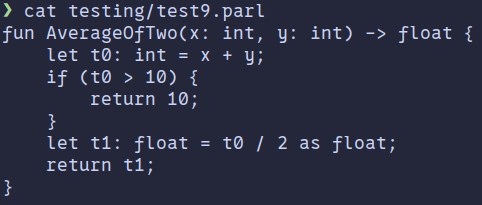
\includegraphics[width=\linewidth]{test9.png}
\caption{\texttt{cat} of the test9.parl}
\label{fig:test9}
\end{figure}

\begin{figure}[H]
\centering
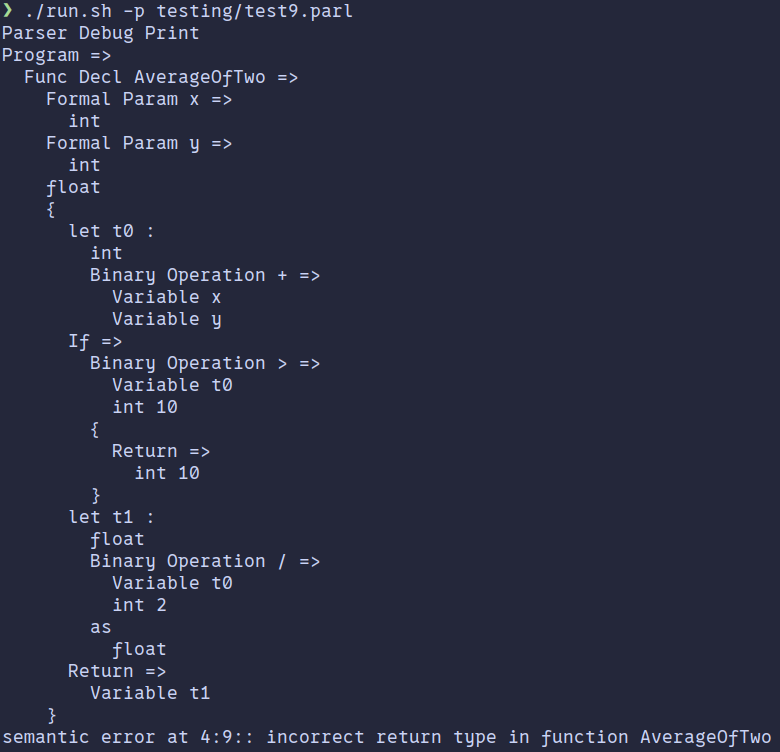
\includegraphics[width=\linewidth]{printervisitoreg.png}
\caption{The AST generated by the syntactically correct program
in test9.parl}
\label{fig:parseeg}
\end{figure}

\lstinputlisting[linerange={104-110}, caption={The
\texttt{debugParsing()} method in the Runner class
(runner/Runner.cpp)},label=lst:debugparsing]{runner/Runner.cpp}

The \texttt{PrinterVisitor} used in \listref{debugparsing} is
a specialization of the pure virtual \texttt{Visitor} class
in parl/Visitor.hpp.

\begin{lstlisting}[caption={A segment of the pure virtual
\texttt{Visitor} class (parl/Visitor.hpp)},
label=lst:genericvisitor]
...

struct ClearStmt;
struct Block;
struct FormalParam;
struct FunctionDecl;
struct IfStmt;
struct ForStmt;
struct WhileStmt;
struct ReturnStmt;
struct Program;

class Visitor {
   public:
    virtual void visit(Type*) = 0;
    virtual void visit(Expr*) = 0;
    virtual void visit(PadWidth*) = 0;
    virtual void visit(PadHeight*) = 0;
    virtual void visit(PadRead*) = 0;
    virtual void visit(PadRandomInt*) = 0;
    virtual void visit(BooleanLiteral*) = 0;
    virtual void visit(IntegerLiteral*) = 0;
    virtual void visit(FloatLiteral*) = 0;

...
\end{lstlisting}

Due to the way \CC{} handles symbols, the classes which the
visitor can visit must be forward declared manually, see
\listref{genericvisitor}. If no such forward declaration is
made, the compiler will complain about the \texttt{Visitor} and
the \texttt{AST} classes being cyclically dependent.

Additionally, any inheriting visitor such as the
\texttt{PrinterVisitor} can hold state. In fact, this is where
the true power of visitors arises. Being able to hold state
means that complex computations can be carried out on the AST.
For example the \texttt{PrinterVisitor} although simple makes
use of a single variable \texttt{mTabCount}, see
\listref{printnode}, which it uses to affect how much
indentation should be used in printing, allowing us to visualise
the AST.

\lstinputlisting[linerange={45-53}, caption={The
\texttt{visit(core::PadRead*)} method in the
\texttt{PrinterVisitor}
(parser/PrinterVisitor.cpp)},label=lst:printnode]{parser/PrinterVisitor.cpp}
